Одним из возможных применений описанной выше задачи является исследование причин возникновения щелей Кирквуда -- определенных областей в поясе астероидов между орбитами Юпитера и Марса, в которых траектории астероидов не могут находиться долгое время. Впервые данные промежутки были обнаружены в 1866 году Д. Кирквудом. Согласно наблюдениям, щели соответствуют целочисленным отношениям периодов орбит астероидов к периоду обращения Юпитера вокруг Солнца. Наиболее отчетливо различимы щели с отношениями: 2:1, 3:1, 5:2, 7:3. 

\begin{figure}[H]
\centering
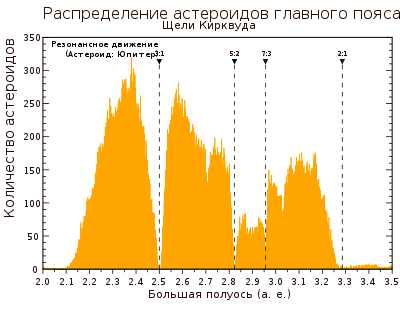
\includegraphics[scale=0.6]{../img/gaps.png}
%\caption{Щели Кирквуда \cite{graph}}
\caption{Щели Кирквуда}

\end{figure}

\begin{figure}[H]
\centering
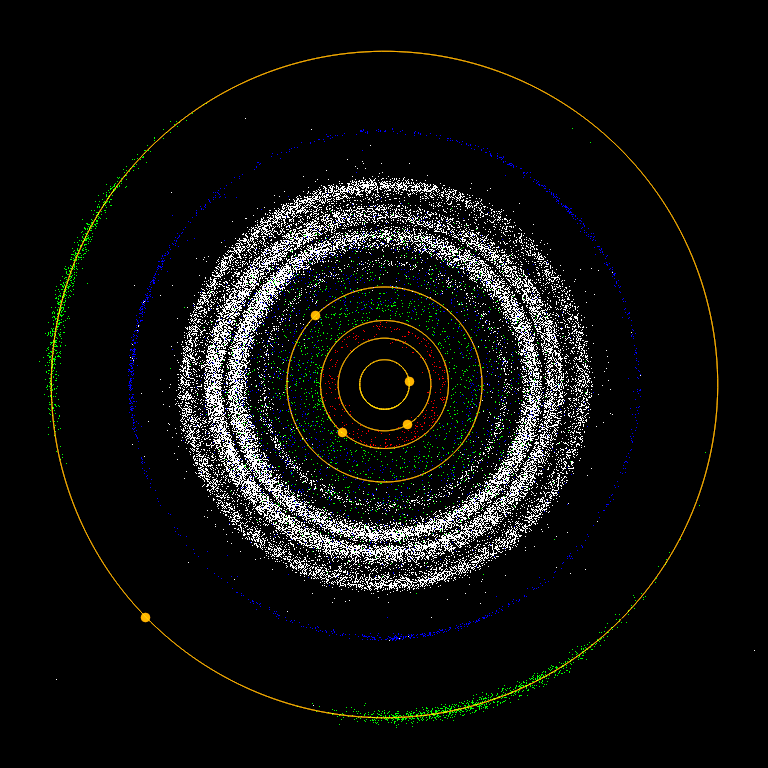
\includegraphics[scale=0.25]{../img/gaps2.png}
%\caption{Астероиды в Солнечной системе \cite{plot}}
\caption{Астероиды в Солнечной системе} 

\end{figure}

Большой вклад в исследование данного вопроса внес Д. Висдом, предложивший использовать метод усреднения для объяснения данного эффекта. Рассмотрим канонические уравнения для описанного выше гамильтониана \cite{wis1}:
\begin{equation}
    \begin{cases}
        \frac{d \Lambda}{dt} = \nu \big( U(x,y) \sin \lambda - V(x,y) \cos \lambda \big), \\
        \frac{d \lambda}{dt} = \alpha \Lambda,\\
        \frac{dx}{dt} = -\nu \left(2Fy+\frac{\partial U(x,y)}{\partial y} \cos \lambda + \frac{\partial V(x,y)}{\partial y} \sin \lambda \right), \\
        \frac{dy}{dt} = \nu \left( 2Fx+e_JG +\frac{\partial U(x,y)}{\partial x} \cos \lambda + \frac{\partial V(x,y)}{\partial x} \sin \lambda \right),
    \end{cases}
    \label{sys2}
\end{equation}
где введены обозначения
$$U(x,y) = C(x^2-y^2)+e_J Dx +e_J^2E,$$
$$V(x,y) = 2Cxy+e_JDy.$$

Так как $\frac{dx}{dt}$ и $\frac{dy}{dt}$ пропорциональны $\nu$, то характерное время изменения переменных $x$ и $y$ имеет порядок $\nu^{-1}$, что заметно больше времени малоамплитудных колебаний $\lambda$ (их характерное время порядка $\nu^{-\frac12}$). В силу этого, $x$ и $y$ можно разделить в сумму длинно- и короткопериодных частей: $x=\overline x + \xi$, $y=\overline y + \eta$, причем длиннопериодная часть описывается усредненной системой уравнений:
\begin{equation}
    \begin{cases}
        \frac{d \overline x}{dt} = -\nu \left( 2F \overline y+\frac{\partial U(\overline x,\overline y)}{\partial \overline y} <\cos \lambda> + \frac{\partial V(\overline x,\overline y)}{\partial \overline y} <\sin \lambda> \right), \\
        \frac{d \overline y}{dt} = \nu \left( 2F \overline x+e_JG +\frac{\partial U(\overline x,\overline y)}{\partial \overline x} <\cos \lambda> + \frac{\partial V(\overline x,\overline y)}{\partial \overline x} <\sin \lambda> \right),
    \end{cases}
\end{equation}
где усреднение идет по периоду колебаний $T$:
$$<\cos \lambda>= \frac{1}{T} \int_0^T \cos \lambda dt = 
    \begin{cases} 
        \frac{2E(k_L)}{K(k_L)} - 1, &  -\sqrt{U^2+V^2} < H < \sqrt{U^2+V^2},\\
        \frac{2E(k_C)}{k_C^2 K(k_C)} + 1 - \frac{2}{k_C^2}, & H < -\sqrt{U^2+V^2},
    \end{cases}$$
$$<\sin \lambda>= \frac{1}{T} \int_0^T \sin \lambda dt = 0,$$
$$
k_L = \sqrt{\frac{\nu \sqrt{U^2+V^2} - H}{2 \nu \sqrt{U^2+V^2}}},\quad
k_C = \sqrt{\frac{2 \nu \sqrt{U^2+V^2}}{\nu \sqrt{U^2+V^2} - H}},
$$
$K(k)$ - полный эллиптический интеграл 1 рода,
$E(k)$ - полный эллиптический интеграл 2 рода.

Метод усреднений позволяет понизить число степеней свободы в полной системе до 1 так, что усредненная система становится интегрируемой в силу наличия интеграла движения - усредненного гамильтониана. 

Несмотря на свои преимущества, данный метод применим не для всех областей фазового пространства. В частности он перестает работать в том случае, когда период колебаний $\lambda$ становится сопоставим с периодами $\overline x$ и $\overline y$. Это происходит когда $\frac{d \lambda}{dt} = O(\nu)$ и, соответственно, сопоставимо с $\frac{dx}{dt}$ и $\frac{dx}{dt}$ в силу малости параметра $\nu$. Таким образом, для траектории системы при каждом прохождении в окрестности нулей функции $U(x,y)\sin \lambda - V(x,y) \cos \lambda$ изменяется значение (квази) адиабатического инварианта действия.